\documentclass[10pt, a4paper, titlepage]{article}
\usepackage[margin=1in]{geometry}
\usepackage{graphicx, latexsym}
\usepackage{titling}
\setlength{\droptitle}{-25em}
\renewcommand{\maketitlehooka}{\Large}
\usepackage{setspace}
\usepackage{amssymb, amsmath, amsthm}
\usepackage[export]{adjustbox}
\usepackage{bm}
\usepackage{wrapfig}
\usepackage{epstopdf}
\usepackage{microtype}
\usepackage[hidelinks]{hyperref}
\usepackage{titling}
\usepackage{multirow}
\usepackage[labelfont=bf]{caption}
\usepackage[table,xcdraw]{xcolor}
\usepackage{colortbl}
\usepackage{lscape}
\usepackage{float}
\usepackage[sort&compress,round,semicolon,authoryear]{natbib}
\hypersetup{
    pdftitle={Research Report Heleen Brüggen},
    pdfauthor={Heleen Brüggen},
    pdfsubject={Research Report Heleen Brüggen},
    pdfkeywords={},
    bookmarksnumbered=true,
    bookmarksopen=true,
    bookmarksopenlevel=1,
    colorlinks=false,
    pdfstartview=Fit,
    pdfpagemode=UseNone
}

\singlespacing

\begin{document}
\begin{titlingpage}
\begin{center}
\Huge\textbf{Master Research Report:  \\ Multilevel Multivariate Imputation by Chained Equations through Bayesian Additive Regression Trees} \\
\Large\textit{Methodology and Statistics for the Behavioural, Biomedical and Social Sciences}

\vspace{.5cm}

\normalsize\textit{Heleen Brüggen}

\vspace{11.5cm}

\begin{minipage}{.5\textwidth}
\begin{center}
        
\includegraphics[width=10cm]{graphs/UU_logo_2021_EN_RGB.png}
\end{center}
\end{minipage}%

\vspace{.25cm}

\begin{minipage}{0.5\textwidth}
\begin{flushleft}

\textbf{Word count:} \\
\textbf{Candidate Journal:} \\
\textbf{FETC Case Number:} \\
\textbf{Supervisors:} \\
MSc. T. Volker \\
Dr. G. Vink \\
MSc. H. Oberman
\end{flushleft}
\end{minipage}%
\begin{minipage}{0.5\textwidth}
\begin{flushright}

2496 \\
Computational Statistics \& Data Analysis \\
23-1778 \\
------------------------\\
Utrecht University \\
Utrecht University \\
Utrecht University
\end{flushright}
\end{minipage}

\end{center}
\end{titlingpage}

\newpage

\section{Introduction}

Incomplete data is a common challenge in many fields of research. Frequently used ad hoc strategies to deal with missing data, such as listwise deletion or mean imputation often lead to erroneous inferences in realistic situations. These strategies don't consider the multivariate nature of the data: the missingness can relate to observed values, which can lead to biased estimates and inaccurate variance estimates \citep{buurenFlexibleImputationMissing2018, kang2013, enders2017, austin2021}. Rubin defined three of such missing data mechanisms: Missing Completely At Random (MCAR) where the cause of the missing data is unrelated to the data, Missing At Random (MAR) where the missing data is related to the observed data, and Missing Not At Random (MNAR) where the missing data may also be related to unobserved data \citep{rubin1976}.

Multiple imputation (MI; \citealt{rubin1987}) is considered a valid method for dealing with incomplete data, it allows us to separate the missing data problem from the analysis problem \citep{mistlerComparisonJointModel2017, buurenFlexibleImputationMissing2018, enders2017, burgette2010, austin2021, audigier2018, vanbuuren2007, grund2021, hughes2014}. MI is used to impute each missing value in the dataset more than once given the observed data, considering necessary variation associated with the missingness problem. The multiply imputed datasets are analyzed, and the corresponding inferences are pooled according to Rubin's rules \citep{buurenFlexibleImputationMissing2018, austin2021, rubin1987, carpenter2013}. However, specifying the imputation models, the models used to impute the missing data, can be challenging. The concept of congeniality dictates that the imputation models should be at least as general as the analysis model and preferably all-encompassing \citep{grund2018, enders2018, meng1994multiple, bartlett2015, grund2016}. Otherwise, it will not capture every aspect of the data and the analysis model estimates may be biased. So, when the complexity of data increases, specifying the imputation models becomes more difficult \citep{grund2018, buurenFlexibleImputationMissing2018}.

Congeniality-issues become more pronounced when MI is used in a multilevel data context \citep{mistlerComparisonJointModel2017, enders2018, enders2018a, enders2020, buurenFlexibleImputationMissing2018, taljaard2008, enders2016, resche-rigon2018, audigier2018, dong2023, grund2016, grund2018a, grund2018, ludtke2017, grund2021, quartagno2022}. Multilevel data is hierarchically structured, where, for example, students are nested within schools \citep{hox2017, hox2011}. When analyzing multilevel data, the hierarchical structure should be considered. Ignoring the hierarchical structure will underestimate the intra-class correlation (ICC; \citealt{buurenFlexibleImputationMissing2018, ludtke2017, taljaard2008, hox2011}), which can be interpreted as the proportion of the total variance at level-2 \citep{gulliford2005, shieh2012, hox2011}. This can be done using multilevel models (MLM; \citealt{hox2017, hox2011, ludtke2017}). MLMs can contain both level-1, and level-2 variables, relating to the individual and class respectively, random intercepts, random slopes, and cross-level interactions \citep{hox2017, hox2011}. Typically, the complexity of the multilevel analysis model is built step-wise with non-linearities, meaning the analysis model is not determined beforehand \citep{hox2017, hox2011}. Thus, including the hierarchical structure, along with the complicated non-linearities from cross-level interactions in imputation models can be quite challenging \citep{buurenFlexibleImputationMissing2018, burgette2010, hox2011} and a very complex model might not converge \citep{buurenFlexibleImputationMissing2018}.

A popular and flexible implementation of MI is fully conditional specification (FCS), otherwise known as chained equations\citep{audigier2018, burgette2010, vanbuuren2007, grund2018a}. FCS iteratively imputes each incomplete variable conditional on complete and previously imputed variables \citep{mistlerComparisonJointModel2017, buurenFlexibleImputationMissing2018, enders2016, enders2018, enders2018a, hughes2014, grund2018a}. In a multilevel context, FCS employs univariate linear mixed models to account for the hierarchical structure \citep{mistlerComparisonJointModel2017, enders2018, resche-rigon2018}. Furthermore, FCS can be used to impute non-linearities, such as cross-level interactions, by using 'passive imputation' or defining a separate imputation model for the non-linearities \citep{buurenFlexibleImputationMissing2018, grund2018}. Still, imputation models including cross-level interaction or non-linear terms in FCS are very complicated \citep{grund2021, grund2018} and, thus, researchers' focus has predominantly been on the inclusion of random intercepts and slopes, but not of cross-level interactions \citep{grund2018a, grund2016, enders2018, enders2018a, enders2020, enders2016}.

Using non-parametric tree-based models might solve this problem because these models do not assume a specific data distribution and, thus, implicitly model non-linear relationships and interactions between the predictor variables, and handle continuous and categorical variables simultaneously \citep{hill2020, burgette2010, lin2019, chipman2010, james2021, salditt2023, breiman1984}. In a single-level imputation context, the use of tree-based, non-parametric models like regression trees, random forests, or Bayesian Additive Regression Trees (BART) simplified imputation models and performed better than parametric methods: the imputations showed better confidence interval coverage of the population parameters, lower variance and lower bias, especially in non-linear and interactive contexts \citep{burgette2010, xu2016, silva2022}. \citet{waljee2013} also found lower imputation error when imputing with a random forest algorithm compared to multivariate imputation by chained equations (\texttt{MICE}), K-nearest neighbors (KNN) and mean imputation.

BART models have been implemented in a multilevel prediction context. However, multilevel-BART models (M-BART) have predominantly been implemented with only random intercepts \citep{chen2020, wagner2020, tan2016, wundervald2022}. In a prediction context, \citet{wagner2020} have found that this random intercept M-BART model provided better predictions with a lower mean squared error (MSE) compared to a parametric MLM, \citet{tan2016} found higher area under the curve (AUC) values compared to a singel-level BART model and linear random intercept model, and \citet{chen2020} found better predictions and better coverage of the estimates compared to parametric models and a single-level BART model. Other researchers modeled the random intercept as an extra split on each terminal node and found a lower MSE compared to a standard BART model and parametric MLMs \citep{wundervald2022}. \citet{dorie2022} developed a multilevel BART model that included random intercepts and random slopes by modeling the random parts with Stan \citep{lee2017} and the fixed parts with BART. Their results showed that their algorithm \texttt{stan4bart} showed better coverage of the population values and lower root mean squared error (RMSE) compared to BART models with varying intercept, BART models ignoring the multilevel structure, bayesian causal forests, and parametric MLMs.

Despite these promising findings, M-BART models have yet to be implemented in a multilevel multiple imputation context. Thus, my thesis research question will be: \textit{Can multivariate imputation by chained equations through a multilevel bayesian additive regression trees model improve the bias, variance, and coverage of the estimates in a multilevel context compared to current practices?} Given the success of non-parametric models in single-level MI, I anticipate that employing M-BART models in a multilevel missing data context will reduce bias, accurately model variance, and improve estimate coverage compared to conventional implementations of multilevel MI, single-level MI, and listwise deletion in the R-package \texttt{MICE} \citep{buuren2011}. However, in this research report, I will only focus on the implementation of M-BART models in a prediction context and asses their performance in terms of relative bias and MSE. The research question is: \textit{Can M-BART models improve the relative bias and MSE of the predictions in a multilevel context compared to a single-level BART model?}.

The research report's sections will cover theoretical background, methods for evaluating M-BART models, preliminary results, and discussion of next steps.

\section{Method}
\subsection{Theoretical background}
\subsubsection{Bayesian Additive Regression Trees (BART)}
BART is a sum-of-trees model proposed by \citet{chipman2010} that has regression trees as its building blocks \citep{chipman2010, hill2020, james2021}. Regression trees divide the data into subgroups by recursively splitting the data into binary subgroups based on the predictors minimizing variability within the subgroups \citep{hastie2017, james2021, salditt2023}. Recursive binary partitioning of the predictor space doesn't assume a specific data form, making this a non-parametric model \citep{hastie2017, james2021, salditt2023} and allows regression trees to model non-linearities well and automatically \citep{hill2020, burgette2010}. \citet{chipman2010} define the BART model as:
\begin{subequations}
\label{eq:BART}
\begin{align}
f(\textbf{x}) &= \sum^{m}_{k=1}g(\textbf{x}; T_{k}, M_{k}), \tag{1}
\end{align}
\end{subequations} where $f(\mathbf{x})$ is the overall fit of the model: the sum of $m$ regression trees, $\textbf{x}$ are the predictor variables, $T_{k}$ is the k\textsuperscript{th} tree and $M_{k}$ is the collection of leaf parameters within the k\textsuperscript{th} tree \citep{chipman2010, hill2020, james2021}. The data are assumed to arise from a model with additive normally distributed errors: $Y = \sum^{m}_{k=1}g(\textbf{x}; T_{k}, M_{k}) + \epsilon, \epsilon \sim \mathcal{N}(0,\,\sigma^{2})$.
Next to the sum-of-trees model, BART also includes a regularization prior that constrains the size and fit of each tree so that each contributes only a small part to prevent overfitting \citep{chipman2010, hill2020, james2021}. BARTs are estimated using the Bayesian back-fitting Markov Chain Monte Carlo (MCMC) algorithm. It updates individual trees, considering the remaining trees, their associated parameters, and the residual standard deviation ($\sigma$). It fits a new tree to the partial residuals, $r_{i}$, treating them as the data, by perturbing the tree from the previous iteration. Perturbations entail either \textit{growing}, \textit{pruning}, or \textit{changing} a tree. \textit{Growing} means adding additional splits, \textit{pruning} removes splits, and \textit{changing} changes decision rules. The algorithm stops after the specified number of iterations. The partial residuals are defined as:
\begin{subequations}
\label{eq:partialresiduals}
\begin{align}
r_i &= y_i - \sum_{k' < k} \hat{f}^{b}_{k'}(x_{i}) - \sum_{k' > k} \hat{f}^{b-1}_{k'}(x_{i}), \text{with } i = 1, \dots, N \tag{2}
\end{align}
\end{subequations} where $\hat{f}^{b}_{k}(x_{i})$ is the prediction of the $k$\textsuperscript{th} tree in the $b$\textsuperscript{th} iteration for person $i$ and sample size $N$.

\subsubsection{Multilevel-BART (M-BART)}
\citet{chen2020, wagner2020} and \citet{tan2016} define a M-BART model including a random intercept building on the work of \citet{lin2019}. The M-BART algorithm breaks down the observed variable into fixed and random components. The fixed components are modeled by BART and the random components are modeled by a linear mixed effects model \citep{chen2020, wagner2020, tan2016}. The BART model (\ref{eq:BART}) can be extended to include a random intercept by:
\begin{subequations}
\label{eq:M-BART}
\begin{align}
f(\textbf{x}) &= \sum^{m}_{k=1}g(\textbf{x}; T_{k}, M_{k}) + \alpha_{j}, \tag{3}
\end{align}
\end{subequations} where, now, $f(\textbf{x})$ is the overall fit of the model incorporating random intercept $\alpha_{j}$ for cluster $j$.

\subsection{Simulation study}
For this research report, I conduct a simulation study to examine the performance of three M-BART models in a multilevel prediction context compared to a single-level BART model.

\subsubsection{Data generating mechanism}
The population data-generating mechanism will be based on the following MLM:
\begin{subequations}
\label{eq:population}
\begin{align}
y_{ij} &= \beta_{0j} + \beta_{1j}X_{1ij} + \beta_{2j}X_{2ij} + \beta_{3j}X_{3ij} + \beta_{4j}X_{4ij} + \beta_{5j}X_{5ij} + \beta_{6j}X_{6ij} + \beta_{7j}X_{7ij} + \epsilon_{ij}, \tag{4} \\
\beta_{0j} &= \gamma_{00} + \gamma_{01}Z_{1j} + \upsilon_{0j}, \tag{4.1} \\
\beta_{1j} &= \gamma_{10} + \gamma_{11}Z_{1j} + \upsilon_{1j}, \tag{4.2} \\
\beta_{2j} &= \gamma_{20} + \gamma_{21}Z_{1j} + \upsilon_{2j}, \tag{4.3} \\
\beta_{3j} &= \gamma_{30} + \gamma_{32}Z_{2j} + \upsilon_{3j}, \tag{4.4} \\
\beta_{4j} &= \gamma_{40} + \upsilon_{4j}, \tag{4.5} \\
\beta_{5j} &= \gamma_{50} + \upsilon_{5j}, \tag{4.6} \\
\beta_{6j} &= \gamma_{60} + \upsilon_{6j}, \tag{4.7} \\
\beta_{7j} &= \gamma_{70}, \tag{4.8}
\end{align}
\end{subequations} where $y_{ij}$ is a continuous level-1 outcome variable for person $i$ in group $j$ and $Z_{1j}$ and $Z_{2j}$ are continuous level-2 variables. The random intercept $\beta_{0j}$ is determined by the grand mean $\gamma_{00}$, the group effect $\gamma_{01}Z_{1j}$ and the group-level random residuals $\upsilon_{0j}$. The regression coefficients $\beta_{1j}$, $\beta_{2j}$, and $\beta_{3j}$ for the continuous variables $X_{1ij}$, $X_{2ij}$, and $X_{3ij}$ depend on the intercepts $\gamma_{10}$, $\gamma_{20}$, and $\gamma_{30}$, the cross-level interactions $\gamma_{11}Z_{1j}$, $\gamma_{21}Z_{1j}$, and $\gamma_{32}Z_{2j}$, and the random slopes $\upsilon_{1j}$, $\upsilon_{2j}$, and $\upsilon_{3j}$. The regression coefficients $\beta_{4j}$, $\beta_{5j}$ and $\beta_{6j}$ are determined by the intercepts $\gamma_{40}$, $\gamma_{50}$ and $\gamma_{60}$ and the random slopes $\upsilon_{4j}$, $\upsilon_{5j}$ and $\upsilon_{6j}$. The regression coefficient $\beta_{7j}$ is determined by the intercept $\gamma_{70}$. The residuals and random slopes $\upsilon_{0j}$, $\upsilon_{1j}$, $\upsilon_{2j}$, $\upsilon_{3j}$, $\upsilon_{4j}$, $\upsilon_{5j}$, and $\upsilon_{6j}$ and $\epsilon_{ij}$ follow a zero-mean normal distribution. The variance of $\upsilon_{0j}$, the group-level random residuals, were scaled such that the specified ICC value as in table \ref{tab:simulationparameters} was obtained. $\upsilon_{1j}$, $\upsilon_{2j}$, $\upsilon_{3j}$, $\upsilon_{4j}$, $\upsilon_{5j}$, and $\upsilon_{6j}$ all have a variance of 1. $\epsilon_{ij}$ had a variance of 25. $X_1$, $X_2$, $X_3$, $X_4$, $X_5$, $X_6$ and $X_7$ are multivariate normally distributed: $\mathbf{X}_{ij} \sim \mathcal{N}(\boldsymbol{\mu}, \boldsymbol{\Sigma})$, with $\boldsymbol{\mu} = (0, 0, 0, 0, 0, 0, 0)$ and $\boldsymbol{\Sigma} = \text{diag}(6.25, 9, 4, 11.56, 4, 2.5, 19.36)$ with no co-variances. The level-2 variables $Z_1$ and $Z_2$ are also multivariate normally distributed:  $\mathbf{Z}_{j} \sim \mathcal{N}(\boldsymbol{\mu}, \boldsymbol{\Sigma})$, with $\boldsymbol{\mu} = (0, 0)$ and $\boldsymbol{\Sigma} = \text{diag}(1, 2.56)$. The group-level effects ($\gamma_{01}$ and $\gamma{02}$) were set to .5, the cross-level interactions ($\gamma_{11}$, $\gamma_{21}$, and $\gamma_{32}$) were set to .35, and the overall intercept ($\gamma_{00}$) was set to 10. The within-group effect sizes ($\gamma_{10}$, $\gamma_{20}$, $\gamma_{30}$, $\gamma_{40}$, $\gamma_{50}$, $\gamma_{60}$, and $\gamma_{70}$) were varied in the simulations.

\subsubsection{Simulation design}
\begin{wraptable}{r}{8cm}
\centering
\caption{Simulation design}
\label{tab:simulationparameters}
\begin{tabular}{l|l}
\textbf{Parameter}                                  & \textbf{Values} \\ \hline
Number of clusters (j)                              & 30, 50          \\
Within-cluster sample size (n\textsubscript{j})     & 5, 15, 35, 50   \\
Intraclass Correlation (ICC)                        & 0, .05, .3, .5  \\
Within-group effect size ($\gamma$)                 & .2, .5, .8
\end{tabular}
\end{wraptable}

Table \ref{tab:simulationparameters} shows the variations considered in the simulation study. They are realistic in practice and/or previously proposed \citep{gulliford1999, murray2003, hox2017, grund2018, enders2018a, enders2020}. For each combination of varying parameters, 6 datasets are simulated to reduce computational time. 4 different models are compared: a single-level BART, single-level BART with groups modelled using dummy-variables, a multilevel BART model incorporating a random intercept \citep{chen2020, wagner2020, tan2016, wundervald2022}, and a multilevel BART model combined with Stan to model the random parts of the models \citep{dorie2022}. The first three models are fitted with the package \texttt{dbarts} \citep{dorie2023} and the last with the package \texttt{stan4bart} \citep{dorie2023a} in R \citep{rcoreteam2023}. The default arguments from the function \texttt{rbart\_vi} are used for all models, as well as the default priors.

\subsubsection{Evaluation}
The fitted models are evaluated in terms of relative bias and Mean Squared Error (MSE) of the predictions \citep{morris2019}:
\begin{subequations}
\label{eq:evaluations}
\begin{align}
\texttt{Bias} &= \frac{1}{n_{\text{sim}}} \sum_{t=1}^{n_{\text{sim}}} (\hat{\theta}_t - \theta), \tag{5} \\
\texttt{MSE} &= \frac{1}{n_{\text{sim}}} \sum_{t=1}^{n_{\text{sim}}} (\hat{\theta}_t - \theta)^{2}, \tag{6} \\
\end{align}
\end{subequations}
where $\hat{\theta}_t$ is the estimated parameter in simulation \textit{t}, $\theta$ is the true value, and $n_{\text{sim}}$ is the number of simulated datasets and smaller is better.

\section{Results}
\graphicspath{{./graphs/}}
Figure \ref{fig:biasplots} shows the average relative bias over the simulations for all models, simulated datasets, every \textit{ICC} value, and within-group effect size. On the x-axis, we can see the different simulated datasets with their names specifying the total sample size, with respectively the number of groups and group sizes within parentheses. We can see that when there is no multilevel structure in the dataset, $ICC = 0$, the models perform similarly in terms of relative bias: overall, the bias is around zero. We can see a slight increase in uncertainty when the total sample size is small for all $\gamma$ and \textit{ICC}. This effect is amplified when $\gamma$ and \textit{ICC} increase. However, when considering the \texttt{stan4bart} model, which models the random parts of the model in Stan and the fixed parts in BART, the uncertainty stays considerably constant when increasing the \textit{ICC}: the relative bias is higher when the total sample size is small, but the uncertainty does not seem to significantly increase with higher \textit{ICC} or higher $\gamma$. Overall, \texttt{stan4bart} has the lowest bias for all $\gamma$ and \textit{ICC} compared to the other models.

\begin{figure}[H]
\caption{Bias of the estimates for all simulated datasets over six simulations with ICC values in the rows and within-group effect sizes in the columns for four models: single-level BART (\texttt{bart}), single-level BART with group dummies (\texttt{gbart}), random intercept multilevel BART (\texttt{rbart}) and random intercept random slope multilevel BART (\texttt{stan4bart}). The x-axis denotes the total sample size (number of groups, group size).}
\centering
\label{fig:biasplots}
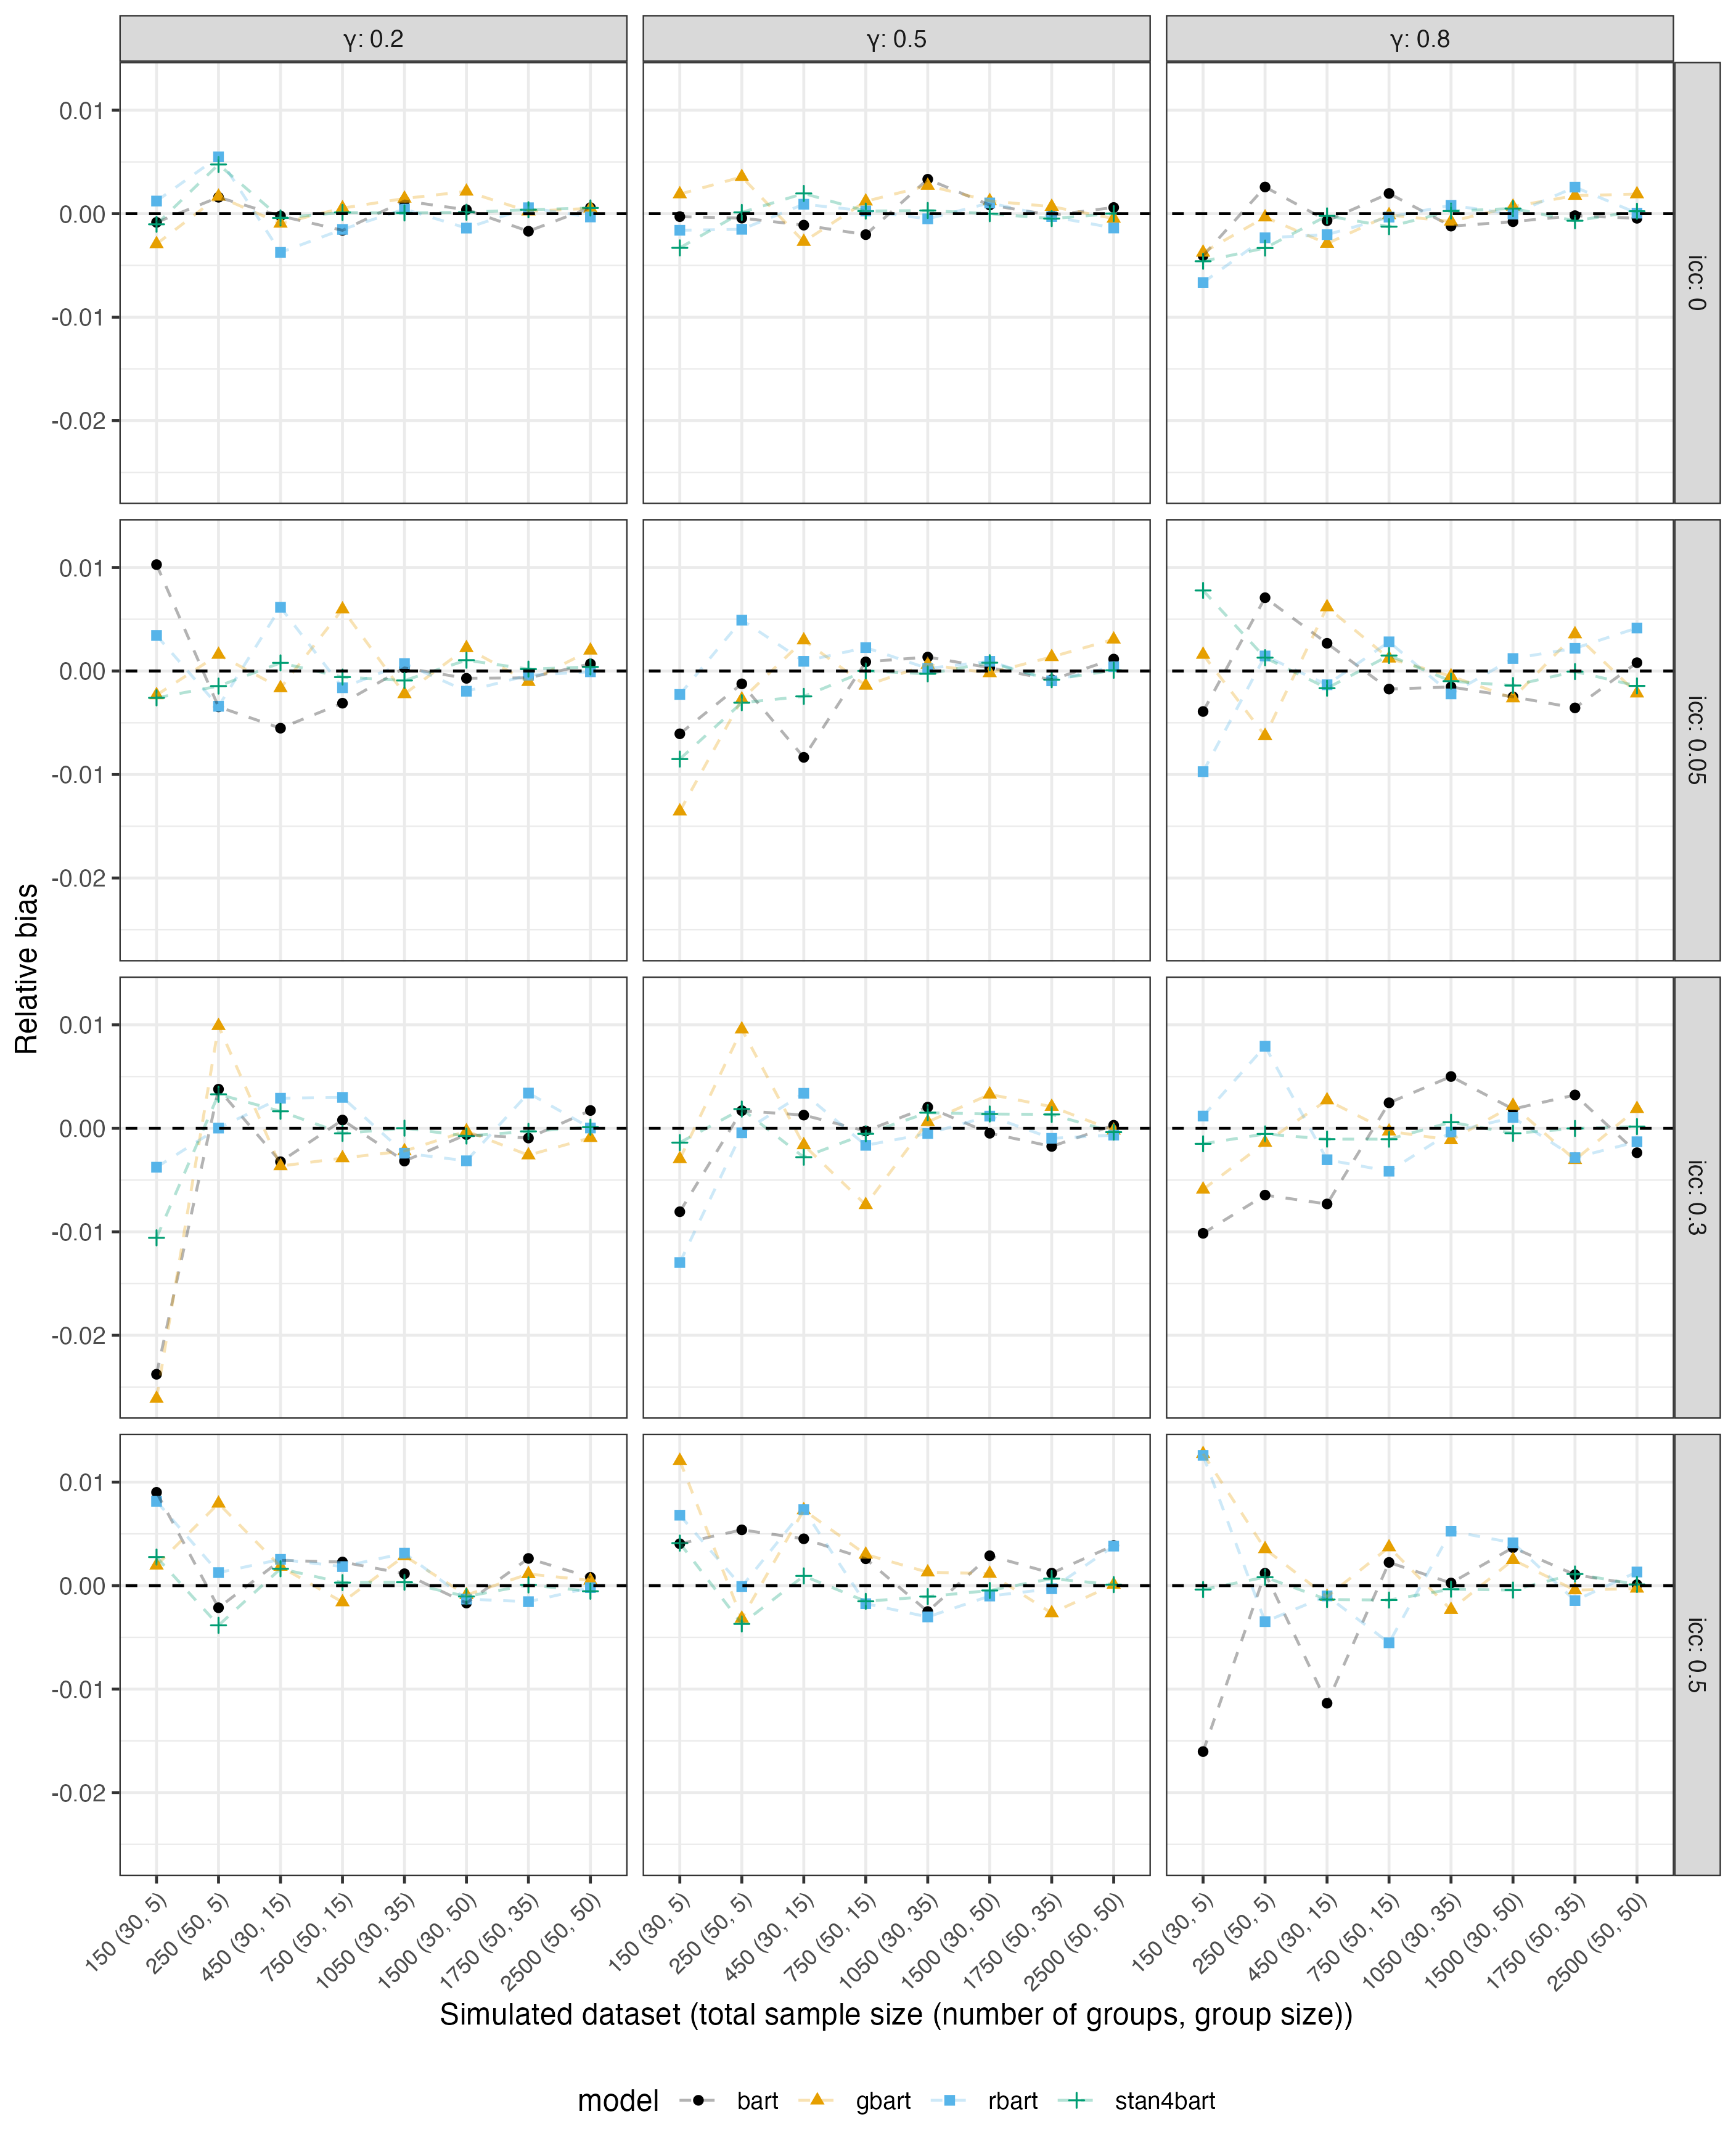
\includegraphics[width=1\textwidth]{biasplot.png}
\end{figure}

Figure \ref{fig:mseplots} shows the average mean squared error (MSE) for all models, datasets, \textit{ICC} values, and within-group effect sizes ($\gamma$). Figure \ref{fig:mseplots} shows that when the $ICC = 0$ the models perform well and almost the same. When increasing the \textit{ICC}, we can start to see a divide in the performance of the models. When $ICC = .05$ the models \texttt{bart}, \texttt{gbart} and \texttt{rbart} perform similarly. Increasing the \textit{ICC} to .3 or .5, the performance of the models separates when the dataset is small: \texttt{bart} now has the highest MSE with \texttt{gbart} performing slightly better. \texttt{rbart} performs better than \texttt{bart} and \texttt{gbart}, but when the datasets increase in size, it performs similarly to them. \texttt{stan4bart} consistently outperforms the other three models in terms of MSE for all \textit{ICC} and $\gamma$ values.

\begin{figure}[H]
\caption{Mean Squared Error (MSE) of the estimates for all simulated datasets over six simulations with ICC values in the rows and within-group effect sizes in the columns for four models: single-level BART (\texttt{bart}), single-level BART with group dummies (\texttt{gbart}), random intercept multilevel BART (\texttt{rbart}) and random intercept random slope multilevel BART (\texttt{stan4bart}). The x-axis denotes the total sample size (number of groups, group size).}
\centering
\label{fig:mseplots}
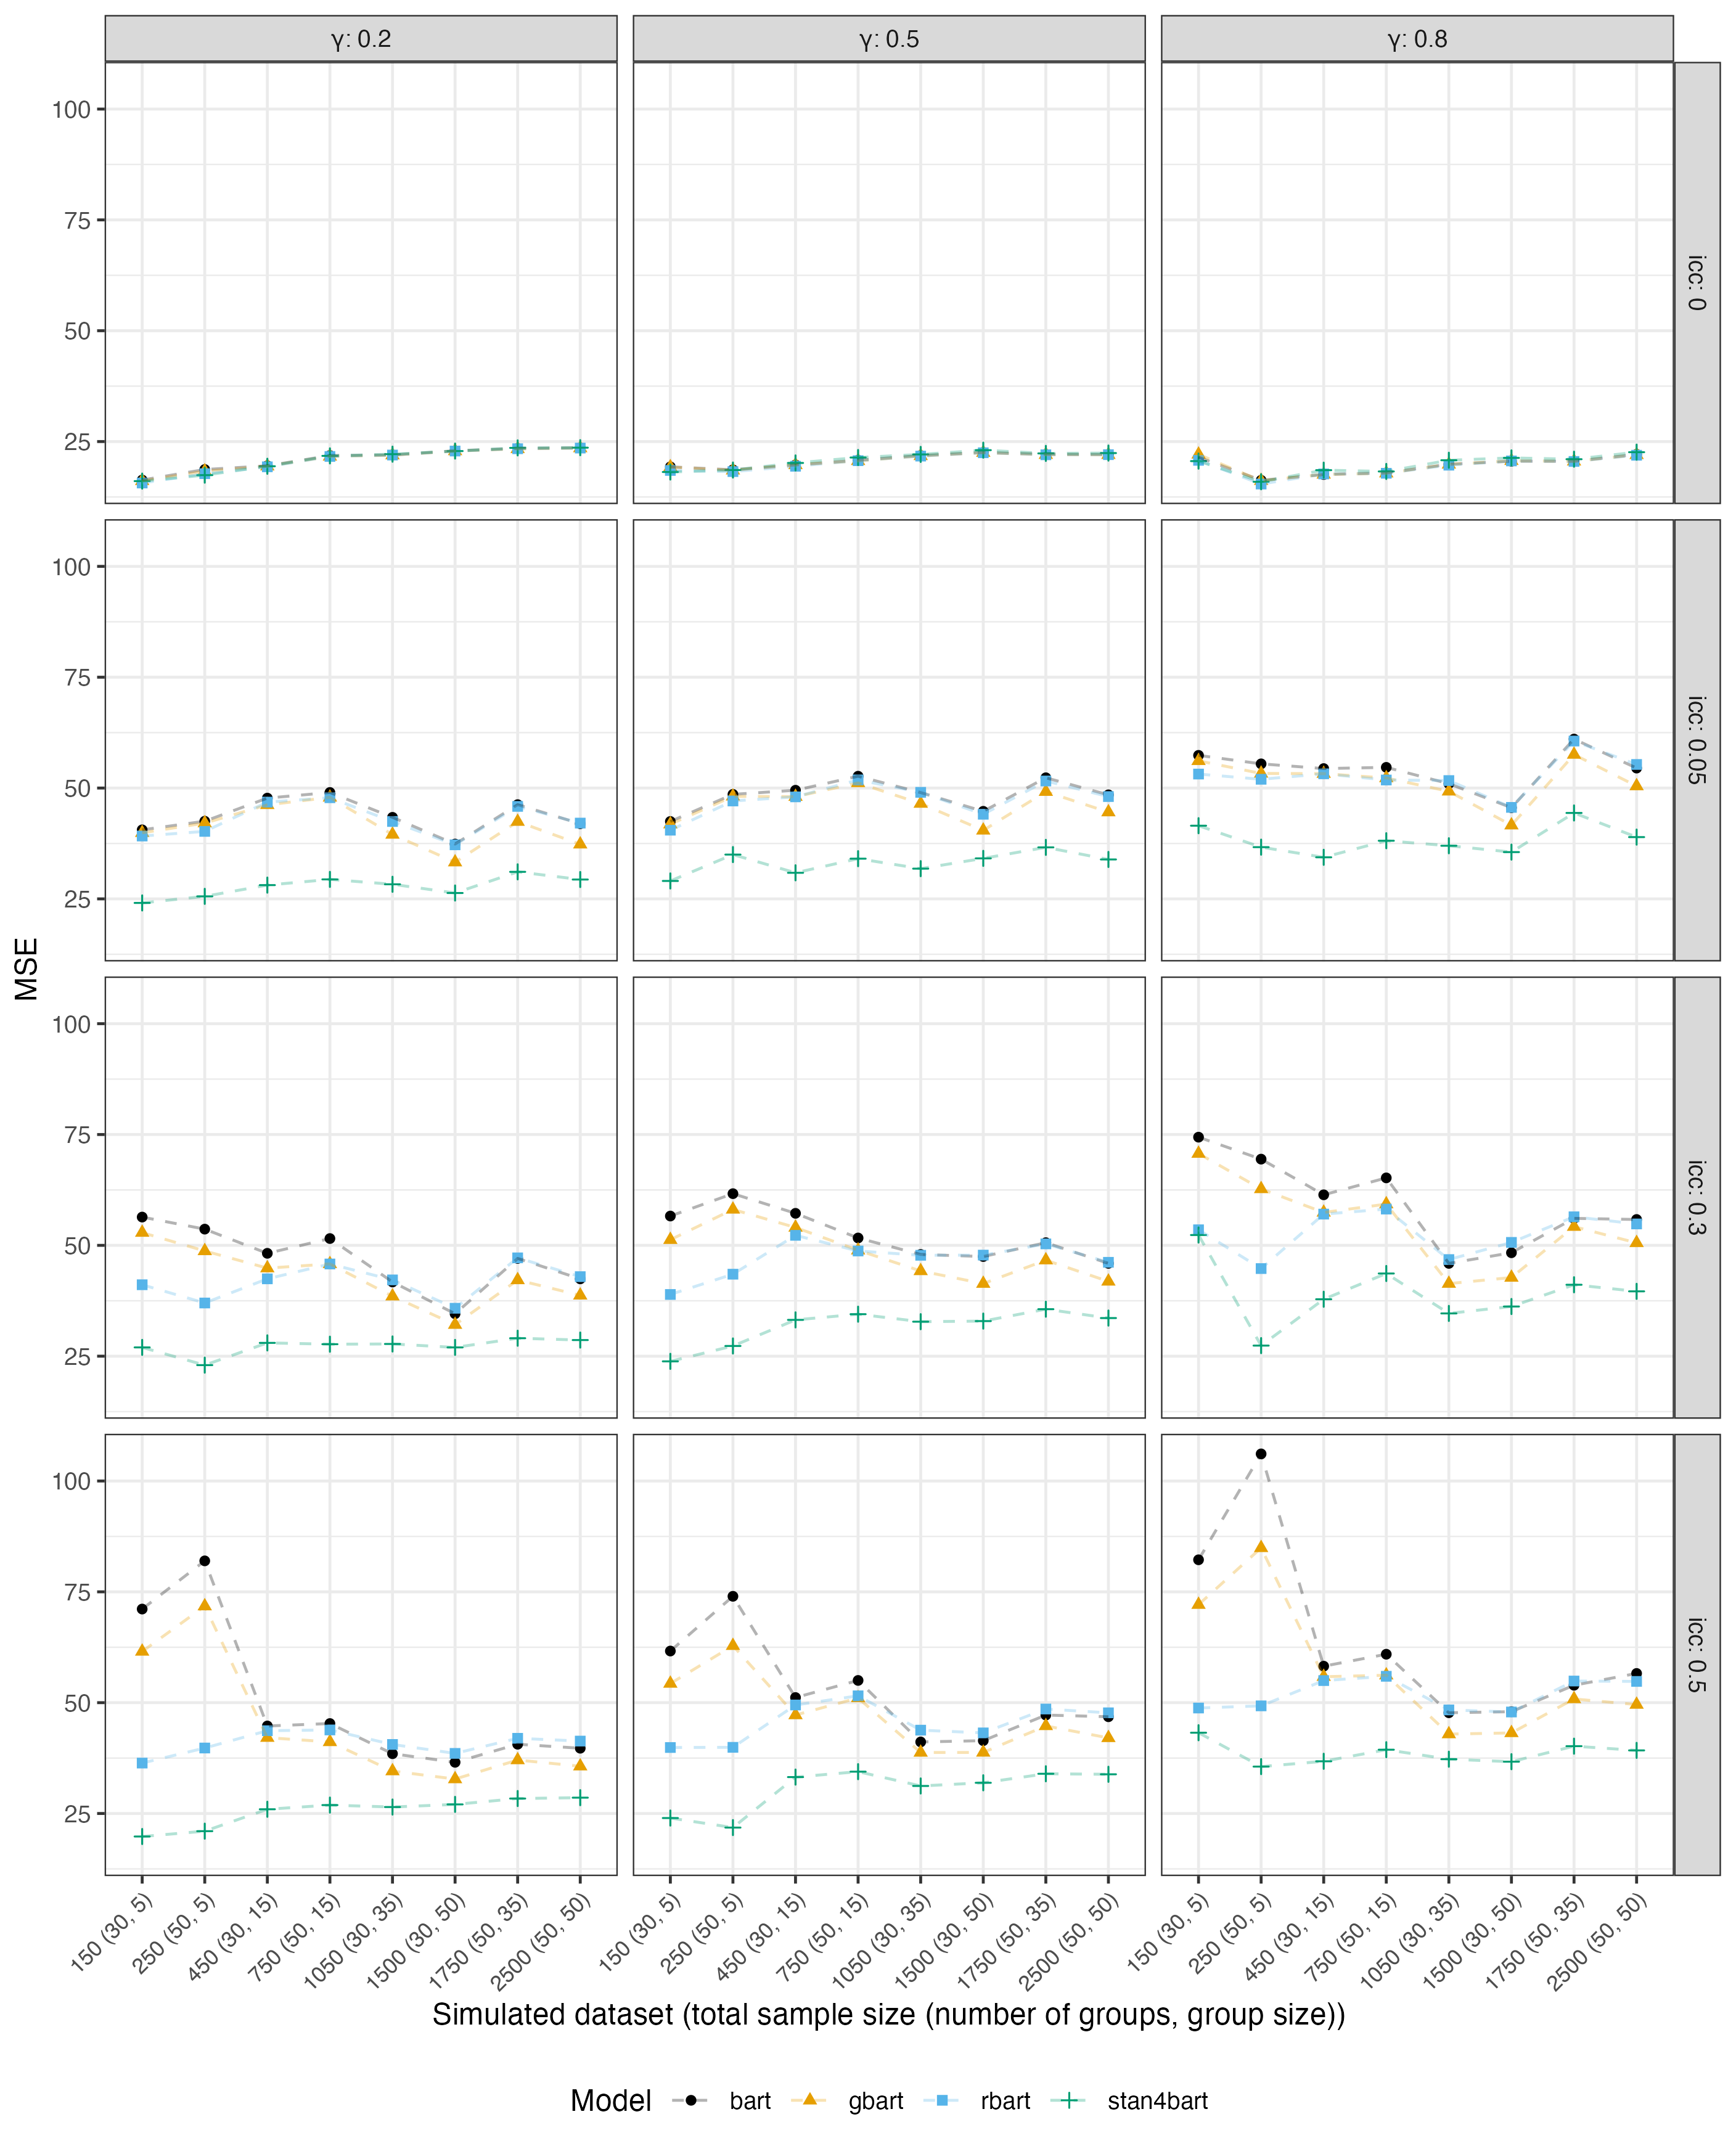
\includegraphics[width=1\textwidth]{mseplot.png}
\end{figure}

\newpage
\section{Discussion}

In this research report, I have investigated the performance of different BART models in terms of relative bias and MSE of the estimates. I considered four different models: a single-level BART model, a single-level BART model including a group-dummy, a multilevel BART model including a random intercept, and a multilevel BART model combining Stan and BART. The results indicate that the \texttt{stan4bart} model performs best out of the four models: it shows to lowest relative bias as well as the lowest MSE. Meaning that, possibly, accounting for more multilevel structure in the model improves it in terms of relative bias and MSE. These results agree with \citet{dorie2022}, who found that the \texttt{stan4bart} algorithm performed better in terms of coverage of the population values and RMSE compared to single-level BART models, BART models including a random intercept, bayesian causal forests, and parametric MLMs.

However, this report has a few limitations. Since I only simulated 6 data sets per scenario to reduce computational constraints, the results might not be fully representative of the performance of the models. Furthermore, I only compared single- and multilevel BART models. Future research could consider bayesian causal forests, other tree-based methods, or parametric MLMs as well. Lastly, I only considered the relative bias and MSE of the predictions but did not consider the relative bias and MSE of the estimated parameters to visualize where the bias is present in the models, which could be interesting in evaluating the performance of the models.

\begin{wraptable}{r}{8cm}
\centering
\caption{Simulation design for the thesis}
\label{tab:simulationparameters2}
\begin{tabular}{l|l}
\textbf{Parameter}                                  & \textbf{Values} \\ \hline
Number of clusters (j)                              & 30, 50          \\
Within-cluster sample size (n\textsubscript{j})     & 5, 15, 35, 50   \\
Intraclass Correlation (ICC)                        & 0, .05, .3, .5  \\
Missing data mechanism                              & MAR, MCAR       \\
Amount of missingness                               & 0\%, 25\%, 50\% \\
Within-group effect size ($\gamma$)                 & .2, .5, .8
\end{tabular}
\end{wraptable}

Building on these results, I will implement the \texttt{stan4bart} as an imputation method within the package \texttt{MICE} \citep{buuren2011} in my thesis. I will compare the performance of the \texttt{stan4bart} model to other imputation methods: \texttt{2l.pmm, 2l.lmer, 2l.pan, 2l.jomo, rf} and single-level \texttt{pmm} and complete case analysis in the R-package \texttt{MICE} \citep{buuren2011}. They will be evaluated in terms of relative bias, modeled variance, and the 95\% confidence interval coverage of the estimates \citep{oberman2023}. The simulation design will be extended to include more parameters: the missing data mechanism and amount of missingness. The simulation design is shown in table \ref{tab:simulationparameters2}. For each combination of parameters, a 1000 replicated datasets will be generated. The preliminary results show great promise for the next steps of my thesis. Hopefully, employing the \texttt{stan4bart} model in a multilevel imputation context will reduce bias, accurately model variance, and improve estimate coverage.

\newpage
\bibliography{thesis}
\bibliographystyle{apalike}

\end{document}

